\documentclass[a4paper,10pt, jcp, aps, preprint]{revtex4-1}

\usepackage[utf8]{inputenc}
\usepackage{amsmath, amsfonts}
\usepackage{graphicx}
\usepackage{natbib}
\usepackage{caption}
\usepackage{subcaption}
\usepackage{authblk}

\bibliographystyle{alpha}

%opening

\author{Rosa Rodríguez \& David P.~Sanders \& W. P. K. Zapfe}
\affil{Departamento de Física, Facultad de Ciencias, Universidad Nacional Autónoma de México, Ciudad Universitaria, Del.~Coyoacán, México D.F. 04510, Mexico}

\usepackage{mathptmx}
% I dont know if that package is compatible with revtex.

\newcommand{\defeq}{:=}
\newcommand{\mean}[1]{\left \langle #1 \right \rangle}
\newcommand{\rd}{\, \mathrm{d}}
\newcommand{\RR}{\mathbb{R}}
\newcommand{\vv}{\mathbf{v}}
\newcommand{\indicator}[1]{\mathbf{1}_{ \{   #1 \} } } 

\setlength{\parskip}{10pt}
\setlength{\parindent}{0pt}

\begin{document}

\title{Exact kinetics of two hard discs in a rectangular box}

\author{Rosa Rodríguez}
\email{sepaeldiablo@notengoidea.org}
\affiliation{unknown to me}

\author{David P. Sanders}
\email{sanders@ciencias.unam.mx}
\affiliation{Facultad de Ciencias, UNAM.}

\author{W. P. Karel Zapfe}
\email{karelz@fis.unam.mx}
\affiliation{Some Cat's Craddle}


\begin{abstract}
  We obtain exact results for the kinetics of the inertial motion of 
two hard discs in a rectangular two-dimensional box.

  In particular,  we calculate exactly the mean hopping time between exchanges
 of the horizontal positions of the discs, 
as well as mean collision rates between the two discs and 
 between the discs and the box. We compare this with numerical experiments.
\end{abstract}

\maketitle

\pmb{NOTE TO DAVID}
I shall use only $r$, \emph{radius} of the disks. To use diameter
means to change all graphics and I am NOT in the mood. Easier to change the notes.
Capital $D$ is for ``dimension''.

\section{Introduction}

Hard sphere billiards are one of the most recurred models in
statistical physics and non linear dynamics.  Some of the simplest models
 provide us with a deep mathematical understanding
about  the properties under the moniker \emph{Hard Chaos} 
(hyperbolicity, ergodicity and mixing qualities). One such system is the
gas of disks in a rectangular box, a two dimensional realisation of a
hard sphere gas. It is known that such a system is chaotic in the
strong sense \cite{Sinai70}. An even simpler realization
is when we take only two disks inside the box, which 
has allready enough degrees of freedom as to make simple representations
of the dynamical system unfeasible. Simplifying it further,
we choose disk of the same radius and mass. The simple
is amenable to analytic treatment of its global qualities,
and rigorous results have been obtain from ergodic theory
\cite{Sinai70, Gallavotti74, SzaszBook00}. 

For the statistical physicist, \emph{mean} and \emph{first} encounter
times are of uttermost importance, as many properties,
such as mixing rates and an interpretative origin of a positive
Liapunov exponent, depend on it. 



\section{Model}

We consider two discs of radius $r$ (and diameter $d=2r$) 
in a box of width $w$ and height $h$ (figure
\ref{billar01}). 
The discs move inertially in the absence of forces, 
following straight line trajectories,
and undergo elastic collisions with each 
other and with the walls of the box.
We take the mass of each disk as $1$, so that the energy
is the value of the Hamiltonian function inside the billiard table:
\begin{equation}
H(q,p)=\frac{1}{2}(\|p_1\|^2+\|p_2\|^2)=1.
\end{equation}

\begin{figure}[h]
  \centering
  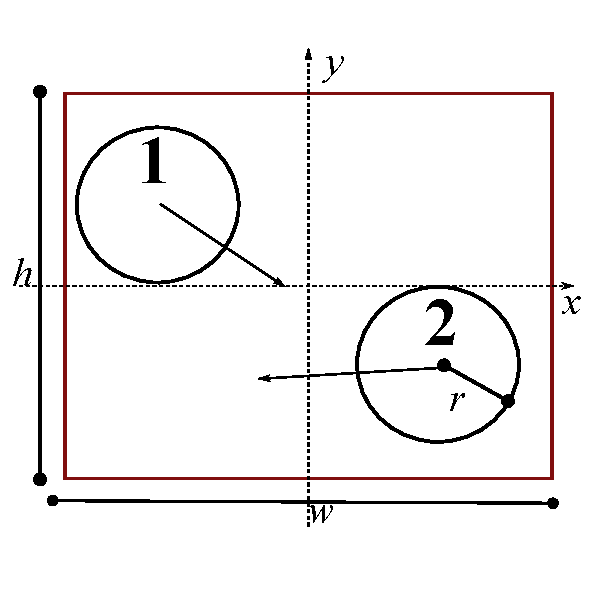
\includegraphics[width=0.56\textwidth]{DiscosenCajaCuadrada01.pdf}
  \caption{The Billiard}\label{billar01}
\end{figure}

We denote the position of the centre of the $i$th disc by 
$(x_{i}, y_{i})$ for $i=1,2$. Since the discs are hard, 
the disc centres are restricted to the region 
$(x_i, y_i) \in [-a,a] \times [-b, b]$, where 
$a \defeq a(r) \defeq \frac{w}{2} - r = \frac{w-d}{2}$ and
 $b \defeq b(r) \defeq \frac{h}{2} - r = \frac{h-d}{2}$.


The exclusion condition is $(x_1-x_2)^2 + (y_1-y_2)^2 \ge (2r)^2 = d^2$.
It is thus useful to work in terms of the new coordinates
\begin{equation}\label{cambiocoor01}
 x \defeq \frac{x_1 - x_2}{\sqrt{2}}; 
\quad X \defeq \frac{x_1 + x_2}{\sqrt{2}}; 
\quad y \defeq \frac{y_1 - y_2}{\sqrt{2}}; 
\quad Y \defeq \frac{y_1 + y_2}{\sqrt{2}}.
\end{equation}


In these coordinates the conditions are rewritten as
$x \in [-a \sqrt{2}, +a \sqrt{2}]$ with 
$X \in [-a \sqrt{2} + |x|, a \sqrt{2} - |x|]$, respectively 
 $y \in [-b \sqrt{2}, b \sqrt{2}]$ and $Y \in [-b \sqrt{2} + |y|, +b \sqrt{2} - |y|]$,  
with the constraint $x^2 + y^2 \ge 2 r^2$.

The exclusions define a hypercube with a hypercylinder inside, placed diagonally 
from one hyperarista to its opposite. 
The dynamics in such a space follow
the usual billiard rules: free flight until
encounter with a wall, then elastic reflection.
The outer borders are flat, so the
hyperbolicity is due only to the inner dispersing
boundary \cite{Sim99}, which represents the collition of
two disks in the original space.


%There are two apparently similar but frustratingly different events.
%If we want to calculate a \emph{Recurrence time} for the collisions 
%between the two disks, 
%we should depart from the subset of all outgoing trajectories from the surface of the
%hyper-cylinder. 
%If we want to calculate the \emph{first} encounter time, then
%this supposition is not necessary.
% Actually, this complicates
%the problem, as there are no general results or 
%techniques to describe this collision in continuous time, and derivations
%imply \emph{continouslly nested integrals}.


\section{Mean time between events}


\subsection{Assumptions for the Collision Rates}

A system of $N$ hard spheres confined by hard walls in a $D$ dimensional
space may be treated as a billiard system 
in which a single point  particle undergoes free motion between reflecting obstacles 
in a $ D N $-dimensional configuration space \cite{Sinai70, MarkChern}. 
If the resulting billiard is ergodic and hyperbolic, then we know that
these systems are equivalent to Bernoulli Flows \cite{Gallavotti74}.
For such systems is expected an exponential decay of 
distributions \cite{AbadiGalves} with potentially
long algebraic tails \cite{ZasTip}. 
This includes recurrence times and
first encounter times. We also
have a result for the mean free time, i.e.\ the mean time between 
collisions of the particle with the walls \cite{MarkChern}. 
This can be thought of as a mean return time to the $(D-1)$-dimensional 
(i.e. co-dimension-$1$) cross-section given by the wall boundaries.
The general formula for that time is
\begin{equation}\label{meanfreetime}
 \mean{\tau} = \frac{|Q|}{|A|} \frac{|S^{D-1}|}{|B^{D-1}|}.
\end{equation}
Here $|Q|$ denotes the $D$-dimensional volume of the available 
space in the billiard and 
$|A|$ the $(D-1)$-dimensional area of the cross-section.
 $|S^{D-1}|$ is the $(D-1)$-dimensional area of the unit sphere in $\RR^D$ given by
\begin{equation}
  |S^{D-1}| = \frac{2 \pi^{D/2}}{\Gamma(D/2)},
\end{equation}
where $\Gamma(\cdot)$ is the gamma function. 
$|B^{D-1}|$ is the volume of the unit ball 
in $\RR^{D-1}$, given by $|B^{D-1}| = |S^{D-2}| / (D-1)$.
In the formula \ref{meanfreetime}  the particle has 
its velocity scaled to unity.

Machta and Zwanzig \cite{MachtaZwan} used a similar method to derive an escape 
time across a non-existent boundary by treating it as a recurrence time.
Since it is an escape time, they used velocities whose components point only 
perpendicularly to the ``exit wall''.

In our case, we are interested in the mean return time to 
a co-dimension-$1$ cross section, 
which is defined by the exact moment
in which the disk interchange their horizontal position. This is simply
\begin{equation} \label{condchoque}
x_1 = x_2.
\end{equation}

Given that each disk has different momentum, but
they can interchange it without affecting the
total energy, we must take into account the mass $m$ of each disk 
and the total kinetic energy $E$.
If both discs have the same mass then $\sum_i \vv_i^2 = 2E / m$.
The above result, as derived by Chernov, 
was for the case $\sum_i \vv_i^2 = 1$, or $m=1$ and $E=\frac{1}{2}$.  
For more general values of $E$ and $m$, 
we are simply working on a different energy surface in phase space. 
The particle trajectories are identical but their motion is a factor
$\sqrt{2E/m}$ faster, so that all times are divided by this value, 
giving for
the mean time between events the general formula:
\begin{equation} \label{meantimegeneral}
  \mean{\tau} =  \frac{1}{\sqrt{2E / m}} 
\frac{|Q| \, |S^3|} {|A| \, |B^3|}.	
\end{equation}
In our particular case, the efective dimension is four,
and $E=m=1$, so that the general factor of the formula appear as:
\begin{equation} \label{meantimegeneralredux}
   \frac{1}{\sqrt{2E / m}} 
\frac{|S^3|}{|B^3|}=\frac{3\pi}{2\sqrt{2}}.	 
\end{equation}

The next step is obtaining the Volume (4 dimensional measure) of
the available space and the Area (3 dimensional induced measure) of
the collision conditions. We devote the next section to
detail the procedure.


\section{Calculation of Volumes and Areas}

The configuration
space is an hypercube with an hyper-cylinder subtracted in a diagonal position.
The uncomfortable part is to deal with the tips of the cylinder, which
present the  shape of a wedge with a circular base and two 
orthogonal ``heights''. 
The calculation can be carried out indirectly, using indicator functions for the
available space or for the  prohibited space.

\subsection{Volume of available space}

We shall present the total four-dimensional volume as a product integral
of all available positions. To better grasp the idea, a convenient
diagram is shown in the figure (\ref{diagintegra01}). Our
principal integral is the avaible free $4D$ volume, which 
we shall denote $V$:
\begin{equation}\label{volindic}
 V = \int_{x_1 = -a}^a \rd x_1 \int_{x_2 = -a}^a \rd x_2 
\int_{y_1 = -b}^b \rd y_1 \int_{y_2 = -b}^b \rd y_2 \, \indicator{ (x_1-x_2)^2 + (y_1-y_2)^2 \ge (2r)^2 },
\end{equation}
where $\indicator{Z}$ indicates the indicator function of the set $Z$, 
given by $\mathbf{1}_Z (x) = 1$ if $x \in Z$, and $=0$ if $x \notin Z$, 
which restricts the integral to the desired region $Z$.

\begin{figure}[h]
  \begin{center}
    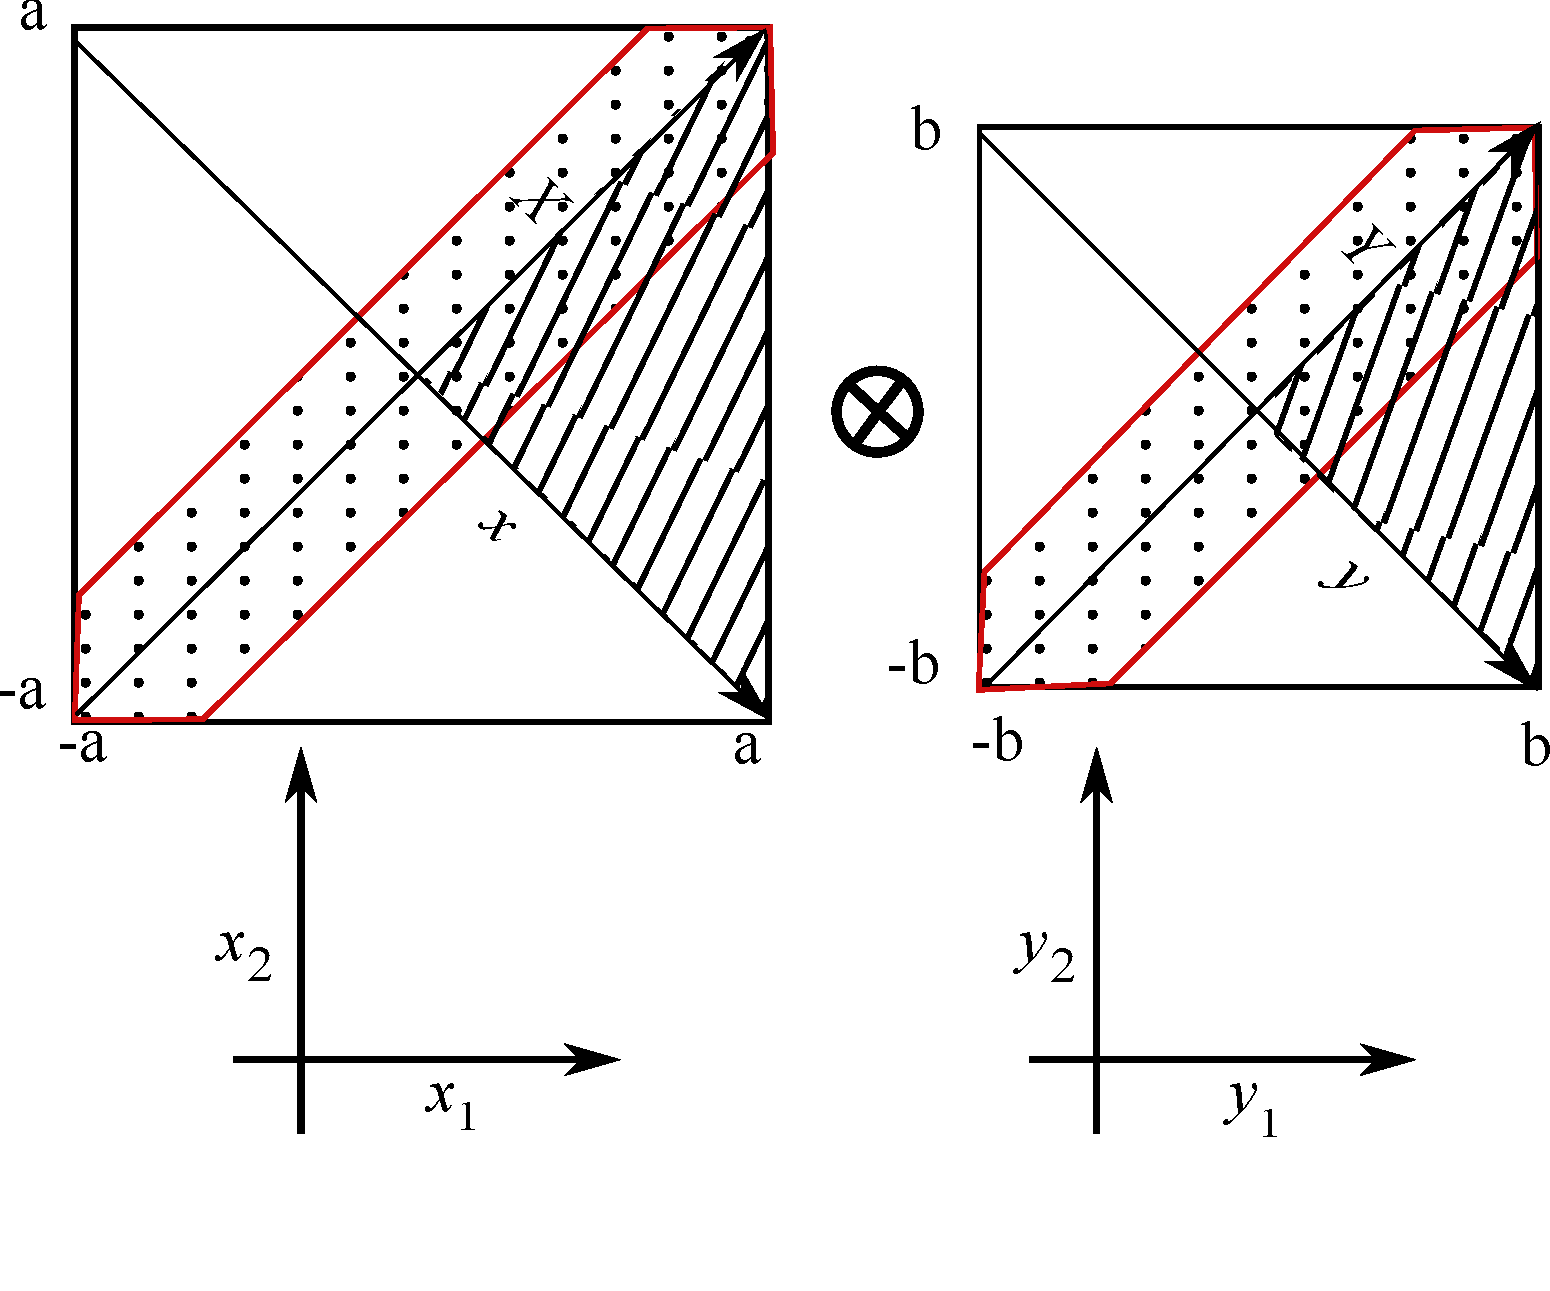
\includegraphics[width=0.75\textwidth]{diagramintegra01.pdf}
    \caption{The space to integrate is the product of the subspaces
      belonging to horizontal and vertical coordinates. The colour
      shaded area represents the ``exclusion'' set, where the condition 
      $ (x_1-x_2)^2 + (y_1-y_2)^2 \ge d^2 $ is not fulfilled. 
      Their width is dependent on the particular point of evaluation
      on the \emph{other} subspace. The diagonal coordinates
      make the expression to evaluate simpler. Due to 
      symmetry, we only evaluate the area in stripes and
      multiply the result by 16.}\label{diagintegra01}
  \end{center}
\end{figure}

We represent the excluded cylinder in the coordinates defined in 
the set of equation \ref{cambiocoor01}. 

\begin{equation}\label{integraltotal}
 V = \int_{x=-a \sqrt{2}}^{a \sqrt{2}} \rd x 
\int_{X=-a \sqrt{2} + |x| }^{a \sqrt{2} - |x|}  \rd X
 \int_{y=-b \sqrt{2}}^{b \sqrt{2}} \rd y
\int_{Y=-b \sqrt{2} + |y| }^{b \sqrt{2}-|y|}  \rd Y
\, \indicator{ x^2 + y^2 \ge 2r^2  }.
\end{equation}
In these coordinates, $X$ and $Y$ do not appear in the integrating part, 
so that these integrals may be done trivially, 
thus reducing to the following two-dimensional integral:
\begin{align}
 V &= \int_{x=-a \sqrt{2}}^{a \sqrt{2}} \rd x  \int_{y=-b \sqrt{2}}^{b \sqrt{2}} \rd y
\, 2 \left( a \sqrt{2} - |x| \right) \, 2 \left( b \sqrt{2} - |y| \right) \,  \indicator{ x^2 + y^2 \ge 2r^2 } \\
&= 16 \int_{x=0}^{a \sqrt{2}} \rd x  \int_{y=0}^{b \sqrt{2}} \rd y
\, \left( a \sqrt{2} - x \right) \, \left( b \sqrt{2} - y \right) \,  \indicator{ x^2 + y^2 \ge 2r^2 },
\end{align}
using the symmetry.
Thus $V = 16(I_1 + I_2)$, where $I_1$ and $I_2$ are the 
resulting integrals over the regions where the available region 
for $y$ is affected by, and is not affected by, respectively, 
the restriction to lie outside the disc.
We have
\begin{align}
 I_1 &= \int_{x=0}^{r\sqrt{2}} \left[ \int_{y = \sqrt{ 2r^2 - x^2}}^{b \sqrt{2}} \left( b \sqrt{2} - y \right) \rd y \right]  \left( a \sqrt{2} - x \right) \rd x \\
&= 	
2 a b^{2} r  + \textstyle \frac{1}{6} (a+b) (2r)^{3} - \frac{1}{32}  (2r)^{4} - \frac{1}{4} {\left(\pi a b + b^{2}\right)} (2r)^2,
\end{align}
and
\begin{align}
 I_2 &= \int_{x=r  \sqrt{2}}^{a \sqrt{2}} \left[ \int_{y = 0}^{b \sqrt{2}} \left( b \sqrt{2} - y \right) \rd y \right]  \left( a \sqrt{2} - x \right) \rd x \\
&=	
{\left( a^{2} - 2ar +   r^{2}\right)} b^{2}.
\end{align}
Thus 
\begin{equation}\label{volumeabd}
 V %= 16(I_1 + I_2) =     	
= 16 a^{2} b^{2}  - 16 \pi a b r^{2} + \textstyle \frac{64}{3} (a+b) r^{3}  - 8 r^{4},
\end{equation}
as was previously obtained by Munakata and Hu \cite{Munakata02}.

Note that the volume available to place two discs inside 
the hard box but \emph{without} the 
 hard-disc exclusion constraint is simply 
given by the first term, $16 a^2 b^2$; 
thus, the remaining terms represent the excluded volume due to this constraint.
The available space gets smaller nevertheless, as can be seen from
the substitutions $a\rightarrow (w-d)/2$ and $b\rightarrow (h-d)/2$.
The explicit formula for the Volume as function from the diameter only is then:
\begin{equation}\label{volumewhd}
 V 
= (w-d)^{2} (h-d)^{2}  - 
 \pi (w-d)(h-d) d^{2} + 
\textstyle \frac{4}{3} (w+h-2d) d^{3}  
- \frac{1}{2} d^{4},
\end{equation}
 
For the numeric values $w=h=1$, the biggest possible radius is 
$r=1/(2+\sqrt{2})$. Unhappily, there is a quirk in the above formula:
it stops being valid before that. The reason is that the deduction
of the formula doesn't include the case in which hopping is not possible. 
We tacitly made the assumption that $h,w>2d$.  This assumption is on 
the integration limits in the step in eq. \ref{integraltotal}. 
A full discussion of the formula for the case in which either
$w$ or $h$ are smaller than $4r$ but there is still space for
the disks is discussed in supplementary material \cite{notascalculokarel}
(\pmb{Appendix?}). 
We cite the  result for $h/4  <r< w/4$ for illustrative purposes.
For cleanliness we define another auxiliary variable,
$c=\sqrt{4r^2-b^2}$:
\begin{multline}\label{VolumenCasoFeo}
V_{h/4<r} = 32abr^2[\arccos(b/2r)-\arccos(a/2r))]\\
+\frac{64 r^3}{3 }[a((b-a)/2r)-b(c/2r+\sqrt{4r^2-a^2}/2r)]\\
-8r^4 [ (b^2-a^2)/4r^2]\\ 
+16[ a b^2 c (4\sqrt{2}-1-\sqrt{2}/3)
+c^2b^2 (\sqrt{2}/3-1) \big]
\end{multline}
In the case that $r$ is larger than both $h/4, w/4$, one must take
into account a similar
contribution which inverts the roles of $a$ and $b$.

In all of our numeric examples we use $w=h=1$, setting the
limit for hops at $r=0.25$. %quite figura redundante del Volumen libre.
We have checked this result with simple Monte Carlo simulations, 
by generating random positions for the disks centres in 
$[-a,a] \times [-b,b]$ uniformly and 
counting the proportion of such initial conditions for 
which the two discs overlap. The fraction of these points to the 
total should give the fraction of prohibited volume over the hypercube
volume. The results are shown in the figure \ref{VolMonteC}.

\begin{figure}[h]
\centering
\includegraphics[width=0.8\textwidth]{VolumenOccupiedByCilinder01.pdf}
\caption{Fraction of occupied volume by the 
Four Dimensional Prohibition Cylinder for the configuration space of the 
Two Disks problems. The red continuous line is formula \ref{volumewhd}, 
which fails after $d>0.5\Leftrightarrow r>0.25$. The numerics
 are forced to follow the adequate behaviour, which is given
by a generalization of the expression \ref{VolumenCasoFeo}. 
 }\label{VolMonteC}
\end{figure}

The following subsections shall only show the formulas for $d<w/2, h/2$.
Bear in mind that some of the dynamics are possible above this limit,
it is only the possition interchange that gets excluded. 

\subsection{Area of cross-section for horizontal interchange (hops), 
$\{x_1 = x_2\}$}

The calculation of the $3$-dimensional area  ( all areas shall be 
denoted by $A$)
of the cross-section 
$\{x_1 = x_2\}$ becomes 
$\{ x=0 \}$ in the new coordinates, proceeds as follows:
\begin{align}
 A_{hopp} &= \int_{X=-a \sqrt{2} }^{a \sqrt{2}}  \rd X
 \int_{y=-b \sqrt{2}}^{b \sqrt{2}} \rd y
\int_{Y=-b \sqrt{2} + |y| }^{b \sqrt{2}-|y|}  \rd Y
\, \indicator{y^2 \ge 2r^2 } \\
&= 8 a \sqrt{2} \int_{y=0}^{b \sqrt{2}} 
\left( b \sqrt{2} - y \right)  \indicator{y \ge r \sqrt{2} }  \rd y \\
&= 8 a \sqrt{2} \int_{y= r\sqrt{2}}^{b \sqrt{2}}  \left( b \sqrt{2} - y \right)  \rd y \\
&= 8 \sqrt{2} a ( b - r )^2. \label{AreaH}
% b^{2} -  b d + \frac{d^{2}}{4} \right) .
\end{align}

We have checked this result with simple Monte Carlo simulations, 
by counting the proportion of successful placements of hard discs 
for which the distance 
$|x_1 - x_2|$ is within a small tolerance of $0$. 
In this case, the possibility to fulfil
the hopping and the non overlapping conditions simultaneously exclude 
all the cases for $\sqrt{2}/(1+\sqrt{2}) <d<1/2$. 
Results are shown in figure \ref{AreaHopp01}.

\begin{figure}[h]
\centering
\includegraphics[width=0.8\textwidth]{AreaHoppChingona02.pdf}
\caption{Here we represent the Volume of a narrow strip around the area
  indicated in the formula in eq. \ref{AreaH}. An $\epsilon$ value acts as
tolerance parameter and produces thus a small volume around the 
hopping condition. By multipling formula \ref{AreaH} by this $\epsilon$
we obtain the teoretical curve shown as a continous line.} 
\label{AreaHopp01}
\end{figure}


\subsection{Area of cross section for collisions}

The area which represents collisions between the two disks is the cylinder area. 
This can be deduced in a similar manner to the free volume, shown in the last
section, or as the derivative of this formula, taking it as as a function evaluated at 
$r\sqrt{2}$. The calculation must be done taking $a,b$ as constants, so that
we do not obtain also the (negative) contribution for the flat ends of
the wedge at the cylinder's end. The resultant area is:
\begin{align}\label{AreaChoque}
A_{collision} & =\sqrt{2}[  
16\pi a b r -32 (a+b)r^2 +16 r^3 ] 
\end{align}

Again, as in eq. \ref{volumewhd}, the formula stops being valid
at $r>0.25$, when the exclusion cylinder has a larger diameter than
the widths or heights of the hypercube.  
We proceed in the same manner as last section, chequing numerically which
random
conditions fall at a small tolerance of $0$ from the Collision Condition, and
plotting this as a fraction of the total volume. The result is shown in the
figure \ref{AreaChoqueTeoyNum}. 

\begin{figure}
\centering
\includegraphics[width=0.8\textwidth]{AreaColision01.pdf}
\caption{The numerical and theoretical calculation for the Area of the cross section
for collision between disks. The plot shows the fraction occupied by a small volume
of size $A_{collision}(r)\times 0.002$ divided by the total
avaible volume $V(r)$. The theoretical formula 
\ref{AreaChoque} breaks down at
$r=1/4$. 
An extra numerical point has been put there to show the deviative behaviour.}
\label{AreaChoqueTeoyNum}.
\end{figure}


\subsection{Area of cross section for  impacts on walls}

For comparison, we shall use also other area to compare
some properties of the decay of time distributions. The most natural choice
would be the mean time between any two collisions. This corresponds
to the adequate measure of the border of the four dimensional
billiard in which the dynamics takes place. This area is
the sum of the area of the hypercilinder and of the border of the
hypercube, taking into consideration the excluded volumen. 
It shall be enough to calculate the cross section area for
the impact of one specific disk unto one specific wall and,
by means of the simmetry of the expressions, obtaining the whole
area. We proced then to calculate the cross section corresponding to 
the disk $1$ hitting the right wall. We acomplish that by
evaluating the next expression in a similar way to
the procedure carried for the expression \ref{volindic}:
\begin{equation}\label{areaindic}
 A_{x_1+} =  \int_{x_2 = -a}^a \rd x_2 
\int_{y_1 = -b}^b \rd y_1 \int_{y_2 = -b}^b \rd y_2 \, \indicator{ (a-x_2)^2 + (y_1-y_2)^2 \ge 4 r^2 }
\end{equation}
The integration procedure is equally tedious, but
straightforward, the result is 
\begin{align}\label{areax1p}
 A_{x_1+} & = 8 a b^2-4  \pi b r^2 +\frac{16}{3}r^3 
 % & = 2(w-d)^2 (h-2)^2- \frac{\pi}{2} (h-d) d^2 +\frac{2}{3}d^3 
\end{align}
Once again, a simple MonteCarlo procedure verifies this result,
shown in fig \ref{area1derecha}. 

\begin{figure}
\centering
\includegraphics[width=0.8\textwidth]{AreaColisionpx1p01.pdf}
\caption{The numerical and theoretical calculation for the cross section area
for the impact of a determined disk with the right wall, as in eq. \ref{areaindic}.
Again, the formula stops being valid at $r>0.25$. }
\label{area1derecha}.
\end{figure}

Given into account the simmetry of the expression for either of 
the disk bouncing in each of the vertical walls, the
cross section area for this event is four times $A_{x_1+}$. On
the other hand, each bounce againsta the horizontal walls would
define a similar quantity, but with the roles of $a$ and $b$ switched.
The cross section area for any impact on the walls would then be:
\begin{align}\label{areawalls}
 A_{walls} & = 32 a b (a+b)-16 \pi r^2 (a+b) +\frac{64\sqrt{2}}{3}r^3 
 %&=  4 (w-d) (h-d)  (w+h-2d) -2 \pi d^2 (w + h-2 d) +\frac{16}{3}d^3. 
\end{align}

The cross section area for any impact or collition 
is then  the sum of the last expression
and the area for collitions between disks, in eq. \ref{AreaChoque}.

\subsection{Area of small hole in a wall}

We can also consider the impact with a very small portion of any of the
walls. If the disks are small enough, this would correspond to an escape time. 
Let us assume a holle of size $\epsilon+2r$ for suitable values of $r$ in
the right side of the wall. Let us assume that the hole is
centered, then the expression to evaluate is
\begin{equation}\label{areaindicagujero}
 A_{x_1+} =  \int_{x_2 = -a}^a \rd x_2 
\int_{y_1 = -b}^b \rd y_1 \int_{y_2 = -b}^b \rd y_2 \, \indicator{ (a-x_2)^2 + (y_1-y_2)^2 \ge 4 r^2 }\indicator{ -\epsilon/2<y_1< \epsilon/2}.
\end{equation}
This would mean that the first disk is hitting the hole. By interchanging the
indexes we would get an equal contribution from the other disk. There is a caveat: 
if the hole or the interaction radius is too large, we have to consider many
more cases for the calculation of the cross section area. The geometry of
the area for integration changes itself according to certain ranges.
We will consider then only small holes. We show a diagram 
in the figure \ref{diagintagu}.
\begin{figure}
\centering
\begin{tabular}{cc}
\includegraphics[width=0.4\textwidth]{diagramintegraagujero01.pdf} &
\includegraphics[width=0.4\textwidth]{diagramintegraagujero02.pdf}
\end{tabular}
\caption{Area of consideration for the integration of expression
 \ref{areaindicagujero}. The left side shows a hole small enough
so that the radius of interacion does not change the geometry of the
indicatrix set, the right side shows the other possibility.}\label{diagintagu}
\end{figure}
The integration is more tedious than in previous examples, as we cannot
take full advantage of the symmetries and we have to split it into
more cases, but still is elemental, and after a good day at the blackboard
it yields
\begin{align}\label{escape}
 A_{escape} &= 2 (w-2r) (h-2r) \epsilon.
\end{align}
\pmb{This is probably wrong.}


\section{Mean times between events}

\subsection{Mean hopping time}

Inserting the results of the previous section 
into the formula for the mean times for crossing
surfaces of section, eq. \ref{meantimegeneral}, gives the times for 
horizontal hopping, 
collition between disks and impacts in general. We use the auxiliary
variables $a,b$ and put everything in terms of $r$. For horizontal
hops we have:
\begin{equation}\label{hoptau}
 \mean{\tau}_{hopp} = 	
\frac{3 \pi}{2\sqrt{2}}
\frac{2 a^{2} b^{2}  - 2 \pi a b r^{2} + \textstyle \frac{a+b}{3}  (2r)^{3}  -  r^4}
{ a \sqrt{2}  ( b - r )^2}.
\end{equation}
The limiting form for very small disk is quite revealling: it is the time
to transverse the distance between two parallel lines at distance $w$ from
a random position, and is related to the Buffon's Needle distribution 
\cite{EScheinerman}:
\begin{equation}\label{hoptaulimit}
 \mean{\tau}_{hopp} \xrightarrow{r\rightarrow 0} 	
\frac{3 \pi}{4}w.
\end{equation}
Also of interest is the limit $r\rightarrow h/4$, where hoping becomes
imposible. The lower term goes to zero as $r^2$ become aproximatelly constant.
This agrees with heuristic arguments. 
In the particular case $w=h$ as in our examples,
seting $r=h/4-\epsilon$ produces the limiting behaviour 
\begin{equation}
 \mean{\tau}_{hopp}(\epsilon) \xrightarrow{\epsilon\rightarrow 0} 	
\frac{3 \pi}{8}
\frac{(1-\frac{2\pi+1}{32})}
{ \epsilon^2} w^3
\end{equation} 

\subsection{Mean collition time}

For the collitions between disk we would have:
\begin{equation}\label{colltau}
 \mean{\tau}_{coll} = 	
\frac{3 \pi}{2\sqrt{2}}
\frac {2 a^{2} b^{2}  - 2 \pi a b r^{2} + \textstyle \frac{a+b}{3}  (2r)^{3}  -  r^4}
{2\pi a b r -4(a+b)r^2+2r^3}
\end{equation}
As expected, this goes to infinity with very small radius, its behaviour
aproaching the expression
\begin{equation}\label{colltaulim0}
\mean{\tau}_{coll}  \xrightarrow{r\rightarrow 0} 
\frac{3}{8\sqrt{2}}\frac{wh}{r}
\end{equation}
On the other side, this should go evaluate to zero when
we use the limiting value for the radius. In the simplest
case  $w = h$ we have $r_{max}= w(\sqrt{2}+2)$. Saddly, our volume
formula ceases to be valid after $r>w/4$, so this limit gives nonsense.
We should go for the more general formula \cite{notascalculokarel}.

\subsection{Mean impact time}

Lastly, for the general impact formula we have the expression:
\begin{equation}\label{impactwall}
 \mean{\tau}_{coll} = 	
\frac{3 \pi}{2\sqrt{2}}
\frac { 2a^{2} b^{2}  -  2\pi a b r^{2} + \frac{a+b}{3}(2r)^3 - r^4}
{ab[8(a+b)+2\pi r]- (4+2\pi)(a+b)r^2+\frac{22}{3} r^3},
\end{equation}
where we have abused from factorization to make the limits clear.

In the limit $r\rightarrow 0$ this goes to $3 \pi (hw)/(8\sqrt{2}(h+w))$.
This should correspond to the average impact time in the walls
for non interacting point particles, 
but, then, ergodic theory would not apply
on such a system. 

\subsection{Mean Sojourn  time for small disks and entrances}

We shall also test the validity of formula using the area in eq. \ref{escape}
for a small holle in the walls. If the formula is to be valid, we have
to make an adecuate balance of the involved parameters. The holle has to
be only marginally larger than the disks, so that they have enough opportunity
to interact, thus achieving \emph{ergodic statistics}. A very large holle
on a wall with similar sized disks will result in only the disk closer to
it escaping. The average escape time then may be calculated as
a return time for the adecuate section and we could use the following formula:
\begin{equation} 
\mean{\tau}_{sojourn} = 	
\frac{3 \pi}{4\sqrt{2}}
\frac {16a^2b^2-16\pi a b r^2 + \frac{64}{3} r^3 - 8 r^2  }
{4 a b \epsilon}.
\end{equation}
As can be expected, this time is proportional to the
free Volume avaible and inversely proportional to the size of the hole, $\epsilon$.
The formula should be adeccuatelly interpreted. This time would represent
the interval that the box, with the afforementioned holle, contains two disks,
starting to count at the moment that the second disks enters the box, and
stoping at the moment any of the disks leaves. 


\section{Numeric Results}

\subsection{Mean hopping time}

We proceed to test last section formulas with
extensive numerical simulations.
The next figure, \ref{MeanHopp01} shows the theoretical curve 
expressed in the formula \ref{hoptau} and some points
that Karel obtained from numerical experiments. A strange unexplained
systematic
deviation has been found. A second analytical curve
has been used for comparition, which uses the volume of the
whole hypercube without taking into account the exluded
set. 

\begin{figure}[h]
  \centering
  \includegraphics[width=0.98\textwidth]{HopTimesPerfect01.pdf}
  \caption{The mean hopping time as function of the radius, Energy, mass, 
and geometry fixed.
The red line is the formula \ref{hoptau}, while the green line
labeled ``Analytical Coarse'' is an approximation using
 $16a^2b^2$ as volume. A logarythmic scale accentuates errors.}\label{MeanHopp01}
\end{figure}

There are many unpleasant characteristics of the figure. First, it must be
noted that even though both numerical and teoretical curves have the
same limit at $r\rightarrow 0$, the slope of the numeric is negative, while 
that of the teoretical curve is positive. The numeric has this weird 
hanged belly until $r\approx 0.125$ which is completely unexplained.

\begin{figure}[h]
        \centering
        \begin{subfigure}[b]{0.45\textwidth}
                \centering
                \includegraphics[width=\textwidth]{HoppingTimesradio01.pdf}
                \caption{$d=0.1$}
                \label{smallradius}
        \end{subfigure}%
        ~ %add desired spacing between images, e. g. ~, \quad, \qquad etc.
          %(or a blank line to force the subfigure onto a new line)
        \begin{subfigure}[b]{0.45\textwidth}
                \centering
                \includegraphics[width=\textwidth]{HoppingTimesRadius249.pdf}
                \caption{$d=0.249$}
                \label{bigradius}
        \end{subfigure}       
        \caption{Histograms for the mean hopping time
in two extreme cases. Left is a very small diameter, while right is an almost
closed pass. While it is not customary to compare logarithmic and non
logarithmic scales, here I take that liberty for the funny features to be
more exaggeratedly shown.}\label{histohopps}
\end{figure}

The figure \ref{bigradius} shows clearly an exponential decay in the
distribution, something to be expected for a chaotic system \cite{OttLibro} , while the
figure in \ref{smallradius} is something different. 

\subsection{Mean collition time}

The results for the collition between the disks are very encouraging. They follow
perfectly the Machta Zwanzig formula, which makes lends credibility to the
strong ergodic hypothesis (figure \ref{MeanHop01}.

\begin{figure}[h]
  \centering
  \includegraphics[width=0.98\textwidth]{CollitionsTime01.pdf}
  \caption{The mean hopping time as function of the radius, Energy, mass, 
    and geometry fixed.
    The red line is the formula \ref{hoptau}, while the green line
    labeled ``Analytical Coarse'' is an approximation using
    $16a^2b^2$ as volume. It can be seen that the numerical results
    are between the two for most of the range.
    A logarithmic scale
    has been used so that sensibility to errors becomes obvious.}\label{MeanHop01}
\end{figure}
 

\subsection{Mean impact time}

The impact against the walls for any discs should follow the expression 
\ref{impactwall}. 

\begin{figure}[h]
  \centering
  \includegraphics[width=0.98\textwidth]{ImpactWallsPerfect01.pdf}
  \caption{The mean hopping time as function of the radius, Energy, mass, 
    and geometry fixed.
    The red line is the formula \ref{hoptau}, while the green line
    labeled ``Analytical Coarse'' is an approximation using
    $16a^2b^2$ as volume. It can be seen that the numerical results
    are between the two for most of the range.
    A logarithmic scale
    has been used so that sensibility to errors becomes obvious.}\label{MeanColl01}
\end{figure}
 

\subsection{Mean sojourn time}


\section{Conclutions}

\section{Aknowledgements}


\bibliography{../../notasmixtas/TwoDiskBiblio}



\end{document}
